\section{PieceWise Linear Discontinuous finite elements}
In this section, we introduce the PieceWise Linear Discontinuous finite
elements developed in \cite{pwld_3d,pwld_2d}. To obtain the PWLD basis
functions on two-dimensional polygons, we need to introduce the within-cell
point $c$. The coordinates of $c$ are weighted averages of the vertex coordinates:
\begin{align}
& x_c = \sum_{j=1}^{V} \alpha_{j} x_j\\
& y_c = \sum_{j=1}^{V} \alpha_{j} y_j
\end{align}
where $\sum_{j=1}^{V} \alpha_{j}=1$, $\alpha_j \geq 0\ \forall j$, and $V$ is 
the number of vertices of the cell.\\
The basis function at vertex $j$ is defined by \cite{pwld_2d}:
\begin{equation}
b_{j} (x,y) = t_{j}(x,y) + \alpha_j t_c(x,y)
\end{equation}
where the $t_j$ functions are the linear functions on the triangle formed
by the three vertices $j-1$, $j$ and $j+1$: $t_j (x,y)$ is unity at vertex $j$
and zero at $j-1$ and $j+1$. The function $t_c(x,y)$ is unity at $c$ 
and zero at each vertex. In this paper, the arbitrary positive weights
$\alpha_j$ are chosen to be $\frac{1}{V}$. On a square cell with 
$\alpha_{j}=0.25\ \forall j$, the basis functions are given in Figure (\ref{pwld}):
\begin{figure}[H]
\centering
\subfloat[First basis function]{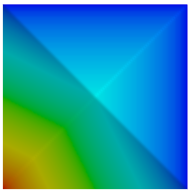
\includegraphics[width=0.25\textwidth]
  {./Spatial_discretizations/pwld_1}}
\subfloat[Second basis function]{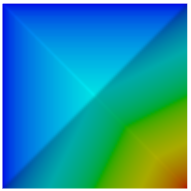
\includegraphics[width=0.25\textwidth]
  {./Spatial_discretizations/pwld_2}}\\
\subfloat[Third basis function]{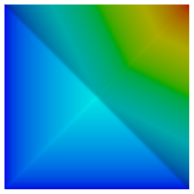
\includegraphics[width=0.25\textwidth]
  {./Spatial_discretizations/pwld_3}}
\subfloat[Fourth basis function]{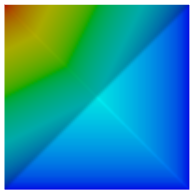
\includegraphics[width=0.25\textwidth]
  {./Spatial_discretizations/pwld_4}}
\caption{PWLD basis function}
\label{pwld}
\end{figure}
On triangular cells, the PWLD basis functions reduces to the standard Linear
Discontinuous (LD) basis functions if $\alpha_j = \frac{1}{3}$. Given the 
definition of the PWLD finite elements, it may seem complicated to build the 
mass matrix, $\bs{M}_{i,j} = \int_{K} b_i(\br) b_j(\br)\ d\br$, or the gradient
matrix, $\bs{G}_{i,j} = \int_K b_j(\br) \bn b_{i}(\br)\ d\br$, on an arbitrary 
polygonal cells. The construction of such matrices can be greatly simplified 
using ``side'' sub-cells. 
A ``side'' sub-cell is a triangular cell made from two adjacent vertices and the 
point $c$. On each ``side'' sub-cells, the mass matrix, for example, can be build
using LD finite elements. The coefficients in the matrix correspondent to the 
point $c$ are shared among the basis function in the cell. For instance, the
mass matrix associated to a quadrilateral cell can be built as follows:\\
First, let us define the mass matrix, $\bs{M}_{PWLD}$, and the mass matrix on a 
``side'' sub-cell $\bs{M}_S$. We assume that the third basis function is associated 
to the middle point of the cell. The first (respectively second) basis function on 
the cell correspond to the first (respectively second) basis function of the 
``side'' sub-cell.
\begin{figure}[H]
  \centering
  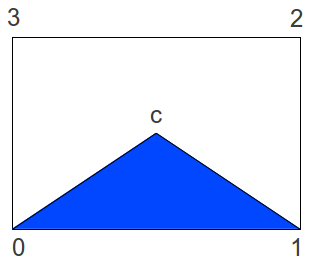
\includegraphics[width=0.3\textwidth]{./Spatial_discretizations/mass_matrix}
  \caption{Sub-cell in the cell}
\end{figure}
Now, $\bs{M}_{PWLD}$ can be filled in using $\bs{M}_S$:
{\allowdisplaybreaks
\begin{align}
  & \bs{M}_{PWLD}(0,0) =  \bs{M}_S(0,0) + \alpha \bs{M}_S(0,2) + \alpha
  \bs{M}_S(2,0) + \alpha^2 \bs{M}_S(2,2)\\
  & \bs{M}_{PWLD}(0,1) =  \bs{M}_S(0,1) + \alpha \bs{M}_S(0,2) + \alpha
  \bs{M}_S(2,1) + \alpha^2 \bs{M}_S(2,2)\\
  & \bs{M}_{PWLD}(0,2) =  \alpha \bs{M}_S(0,2) + \alpha^2 \bs{M}_S(2,2)\\
  & \bs{M}_{PWLD}(0,3) =  \alpha \bs{M}_S(0,2) + \alpha^2 \bs{M}_S(2,2)\\
  & \bs{M}_{PWLD}(1,0) =  \bs{M}_S(1,0) + \alpha \bs{M}_S(1,2) + \alpha
  \bs{M}_S(2,0) + \alpha^2 \bs{M}_S(2,2)\\
  & \bs{M}_{PWLD}(1,1) =  \bs{M}_S(1,1) + \alpha \bs{M}_S(1,2) + \alpha
  \bs{M}_S(2,1) + \alpha^2 \bs{M}_S(2,2)\\
  & \bs{M}_{PWLD}(1,2) =  \alpha \bs{M}_S(1,2) + \alpha^2 \bs{M}_S(2,2)\\
  & \bs{M}_{PWLD}(1,3) =  \alpha \bs{M}_S(1,2) + \alpha^2 \bs{M}_S(2,2)\\
  & \bs{M}_{PWLD}(2,0) =  \alpha \bs{M}_S(2,0) + \alpha^2 \bs{M}_S(2,2)\\
  & \bs{M}_{PWLD}(2,1) =  \alpha \bs{M}_S(2,1) + \alpha^2 \bs{M}_S(2,2)\\
  & \bs{M}_{PWLD}(2,2) =  \alpha^2 \bs{M}_S(2,2)\\
  & \bs{M}_{PWLD}(2,3) =  \alpha^2 \bs{M}_S(2,2)\\
  & \bs{M}_{PWLD}(3,0) =  \alpha \bs{M}_S(2,0) + \alpha^2 \bs{M}_S(2,2)\\
  & \bs{M}_{PWLD}(3,1) =  \alpha \bs{M}_S(2,1) + \alpha^2 \bs{M}_S(2,2)\\
  & \bs{M}_{PWLD}(3,2) =  \alpha^2 \bs{M}_S(2,2)\\
  & \bs{M}_{PWLD}(3,3) =  \alpha^2 \bs{M}_S(2,2)
\end{align}}    
By looping over all the ``side'' sub-cell of a cell, the mass matrix of the 
cell can be easily built. The gradient matrix can be built similarly.
